
\section{Blitzerdung}
\label{section:blitzerdung}
\begin{frame}%STARTCONTENT
\begin{itemize}
  \item Antennenanlagen erhöhen nicht die Wahrscheinlichkeit für einen Blitzeinschlag
  \item Wenn aber ein Blitz einschlägt, dann in die exponierte Antenne
  \item Deshalb müssen \emph{Antennenanlagen geerdet} oder in ein vorhandenes \emph{Blitzschutzkonzept} integriert werden
  \end{itemize}

\end{frame}

\begin{frame}
\frametitle{Überspannung}
\begin{columns}
    \begin{column}{0.48\textwidth}
    
\begin{figure}
    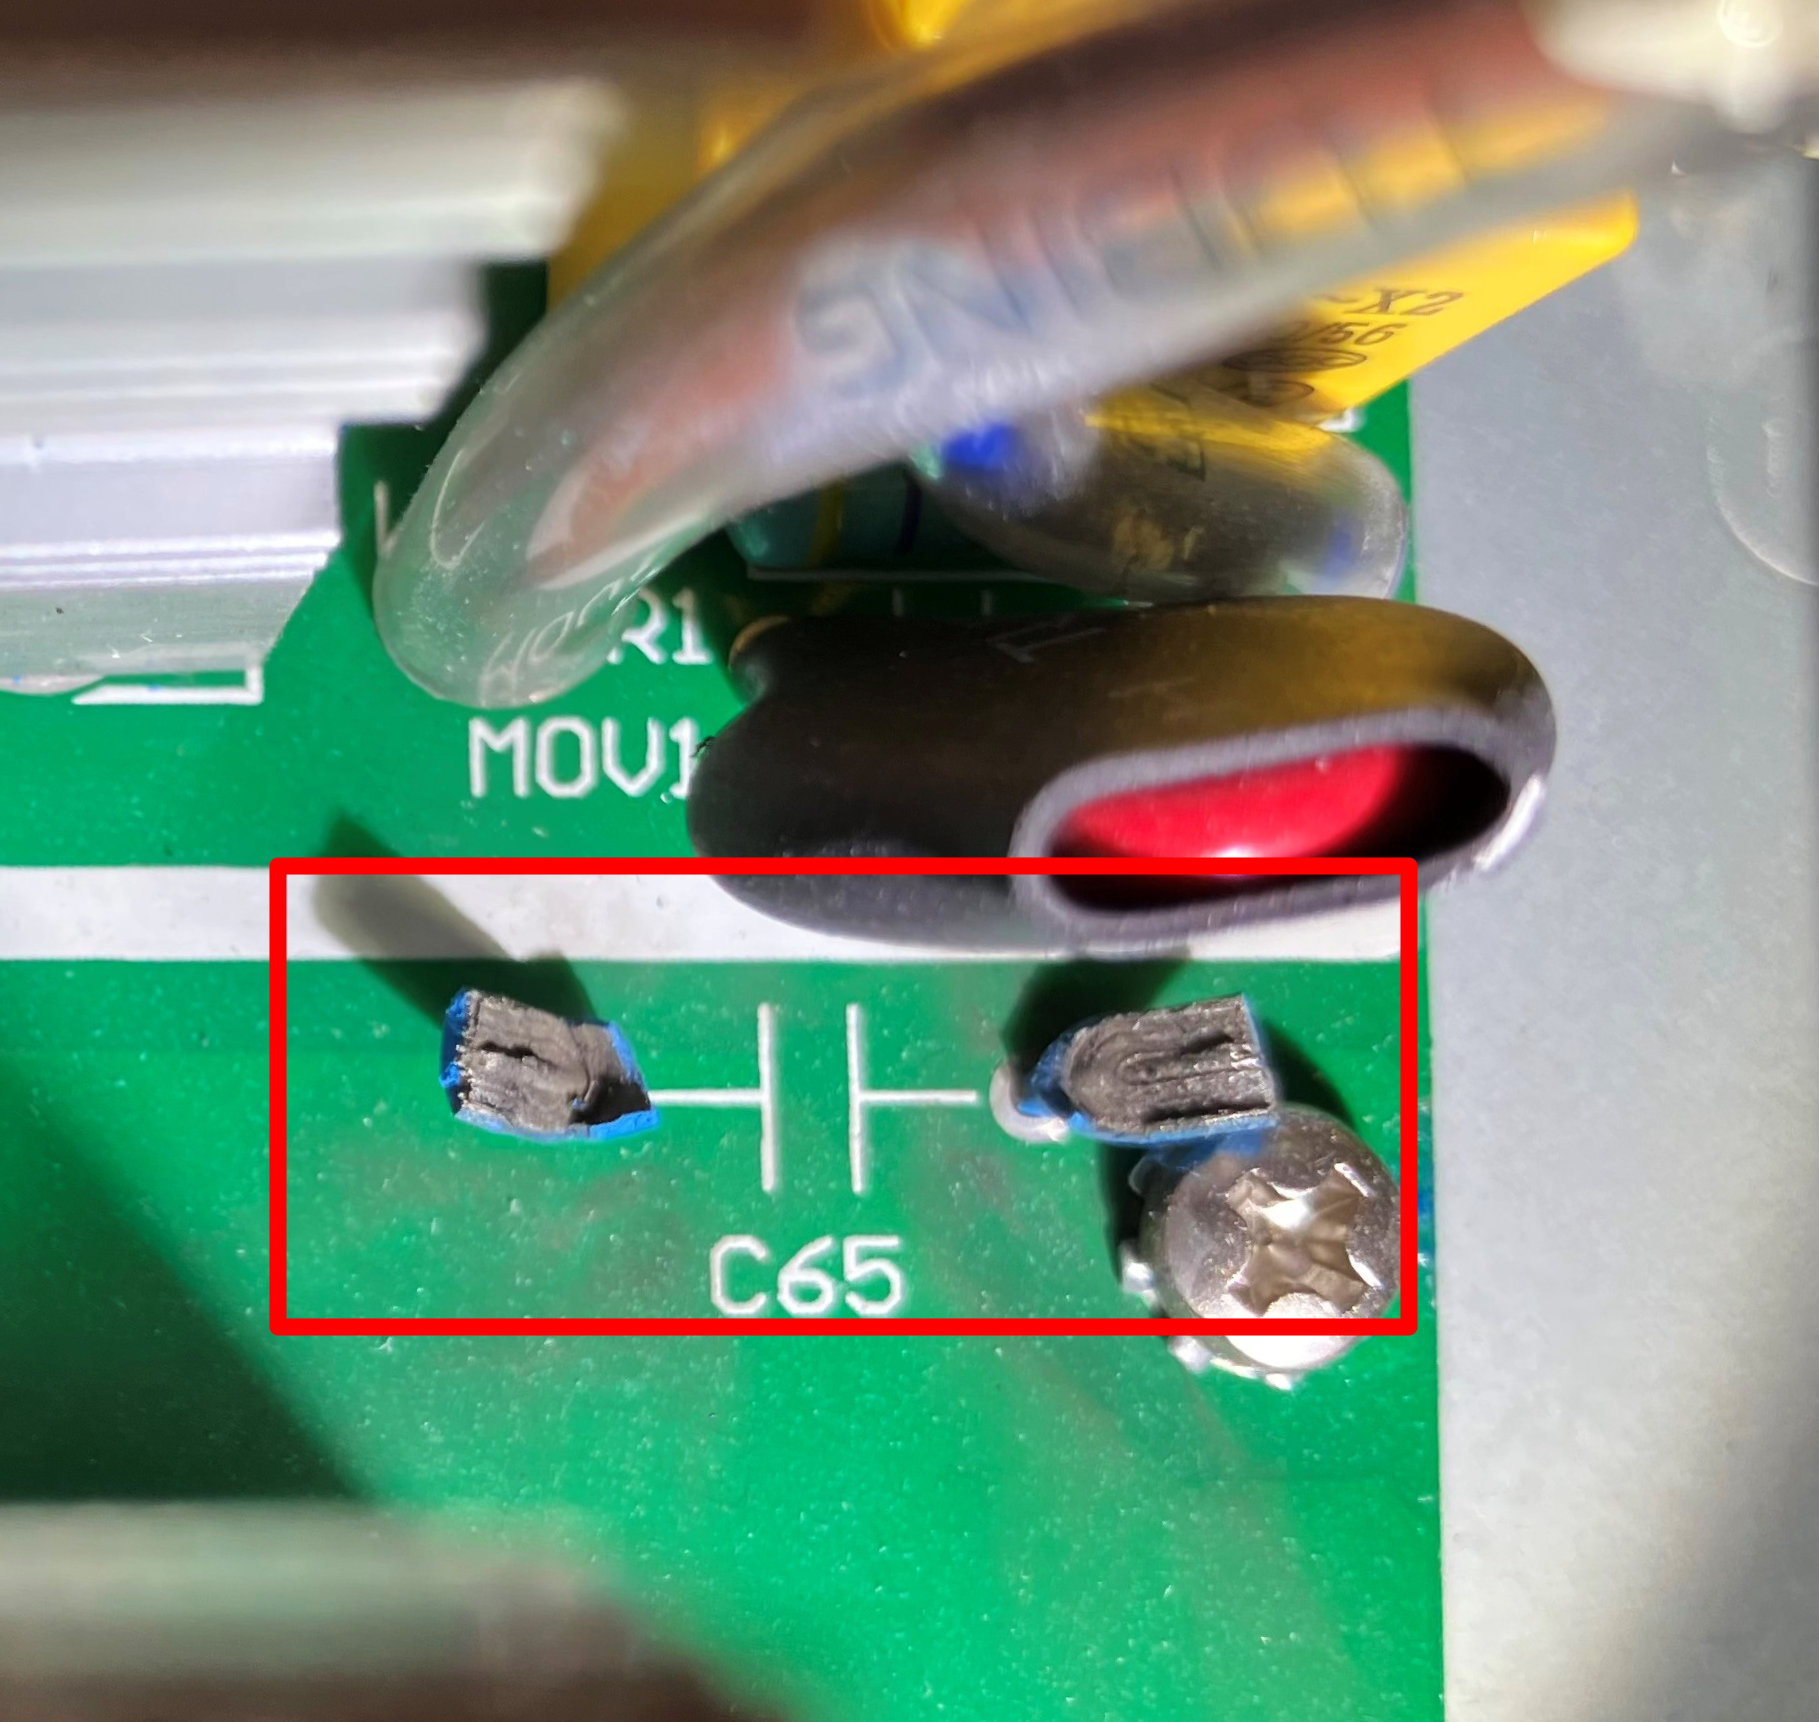
\includegraphics[width=0.85\textwidth]{foto/191}
    \caption{\scriptsize Durch Überspannung völlig zerstörter Kondensator in einem Netzteil. Ursache war ein Blitzeinschlag in der Nähe der Station. Hier kam die Überspannung über das Stromnetz.}
    \label{}
\end{figure}

    \end{column}
   \begin{column}{0.48\textwidth}
       \begin{itemize}
  \item Auch ein Blitz in der Nähe kann durch Überspannung große Schäden anrichten
  \item Ursache ist Induktion in Strom- oder Telefonienetz
  \end{itemize}

   \end{column}
\end{columns}

\end{frame}

\begin{frame}
\frametitle{Blitzschutz}
\begin{columns}
    \begin{column}{0.48\textwidth}
    \begin{itemize}
  \item Blitzschutz-Zwischenstecker für Koaxialkabel mit Gasentladungsröhre
  \item Antennenzuleitung nach dem Funkbetrieb erden, z.B. an Gebäudeerdungsanlage
  \item Dafür ist eine Erdungsleitung notwendig
  \end{itemize}

    \end{column}
   \begin{column}{0.48\textwidth}
       \begin{itemize}
  \item Massiver Draht, keine Litze
  \item Kupfer \qty{16}{\milli\metre}<sup>2</sup>
  \item Aluminium \qty{25}{\milli\metre}<sup>2</sup>
  \item Stahl \qty{50}{\milli\metre}<sup>2</sup>
  \end{itemize}

   \end{column}
\end{columns}

\end{frame}

\begin{frame}
\only<1>{
\begin{QQuestion}{EK209}{Unter welchen Bedingungen darf eine Gebäudeerdungsanlage für die Antennenerdung verwendet werden?}{Jede Gebäudeerdungsanlage kann verwendet werden.}
{Für jede Antenne muss eine separate Erdungsanlage unabhängig von der Gebäudeerdungsanlage aufgebaut werden.}
{Wenn die Gebäudeerdung vom Prüf- und Messdienst der Bundesnetzagentur abgenommen wurde.}
{Die Antennenanlage darf nicht über die von der Gebäudeerdungsanlage eingeschlossenen Fläche hinausragen.}
\end{QQuestion}

}
\only<2>{
\begin{QQuestion}{EK209}{Unter welchen Bedingungen darf eine Gebäudeerdungsanlage für die Antennenerdung verwendet werden?}{\textbf{\textcolor{DARCgreen}{Jede Gebäudeerdungsanlage kann verwendet werden.}}}
{Für jede Antenne muss eine separate Erdungsanlage unabhängig von der Gebäudeerdungsanlage aufgebaut werden.}
{Wenn die Gebäudeerdung vom Prüf- und Messdienst der Bundesnetzagentur abgenommen wurde.}
{Die Antennenanlage darf nicht über die von der Gebäudeerdungsanlage eingeschlossenen Fläche hinausragen.}
\end{QQuestion}

}
\end{frame}

\begin{frame}
\only<1>{
\begin{QQuestion}{EK210}{Welches Material und welcher Mindestquerschnitt kann für eine Erdungsleitung zwischen einem Antennenstandrohr und einer Erdungsanlage nach VDE~0855-300 beispielsweise verwendet werden?}{Ein- oder mehrdrähtiger - aber nicht feindrähtiger - Leiter aus Kupfer~(\qty{10}{\mm\squared}) oder Aluminium~(\qty{16}{\mm\squared}).}
{Einzelmassivdraht aus Kupfer~(\qty{16}{\mm\squared}), Aluminium~(\qty{25}{\mm\squared}) oder Stahl~(\qty{25}{\mm\squared}).}
{Einzelmassivdraht aus Kupfer~(\qty{16}{\mm\squared}), Aluminium~(\qty{25}{\mm\squared}) oder Stahl~(\qty{50}{\mm\squared}).}
{Ein- oder mehrdrähtiger - aber nicht feindrähtiger - Leiter aus Kupfer~(\qty{4}{\mm\squared}) oder Aluminium~(\qty{10}{\mm\squared}).}
\end{QQuestion}

}
\only<2>{
\begin{QQuestion}{EK210}{Welches Material und welcher Mindestquerschnitt kann für eine Erdungsleitung zwischen einem Antennenstandrohr und einer Erdungsanlage nach VDE~0855-300 beispielsweise verwendet werden?}{Ein- oder mehrdrähtiger - aber nicht feindrähtiger - Leiter aus Kupfer~(\qty{10}{\mm\squared}) oder Aluminium~(\qty{16}{\mm\squared}).}
{Einzelmassivdraht aus Kupfer~(\qty{16}{\mm\squared}), Aluminium~(\qty{25}{\mm\squared}) oder Stahl~(\qty{25}{\mm\squared}).}
{\textbf{\textcolor{DARCgreen}{Einzelmassivdraht aus Kupfer~(\qty{16}{\mm\squared}), Aluminium~(\qty{25}{\mm\squared}) oder Stahl~(\qty{50}{\mm\squared}).}}}
{Ein- oder mehrdrähtiger - aber nicht feindrähtiger - Leiter aus Kupfer~(\qty{4}{\mm\squared}) oder Aluminium~(\qty{10}{\mm\squared}).}
\end{QQuestion}

}
\end{frame}

\begin{frame}
\frametitle{Blitzschutzkonzept}
\begin{itemize}
  \item Bei Änderungen an der Blitzschutzanlage eine Blitzschutz-Fachkraft einbeziehen
  \item Insbesondere beim Anschluss von Antennen-Standrohren an die Blitzschutzanlage
  \item Aufnahme der Veränderungen in das Blitzschutzkonzept des Gebäudes
  \end{itemize}
\end{frame}

\begin{frame}
\only<1>{
\begin{QQuestion}{EK211}{Unter welchen Bedingungen darf das Standrohr einer Amateurfunkantenne auf einem Gebäude mit dem gebäudeeigenen Blitzschutzsystem verbunden werden?}{Wenn eine Blitzschutz-Fachkraft die Verbindung des Standrohres der Amateurfunkantenne mit dem Blitzschutzsystem im Blitzschutzkonzept vorsieht.}
{Nach den geltenden Vorschriften muss das Standrohr der Amateurfunkantenne mit einem Gebäudeblitzschutzsystem verbunden werden.}
{Nach den geltenden Vorschriften muss immer ein getrenntes Blitzschutzsystem für die Amateurfunkantenne aufgebaut werden.}
{Wenn für die Verbindungsleitung ein Kupferleiter mit ausreichend großem Querschnitt verwendet wird.}
\end{QQuestion}

}
\only<2>{
\begin{QQuestion}{EK211}{Unter welchen Bedingungen darf das Standrohr einer Amateurfunkantenne auf einem Gebäude mit dem gebäudeeigenen Blitzschutzsystem verbunden werden?}{\textbf{\textcolor{DARCgreen}{Wenn eine Blitzschutz-Fachkraft die Verbindung des Standrohres der Amateurfunkantenne mit dem Blitzschutzsystem im Blitzschutzkonzept vorsieht.}}}
{Nach den geltenden Vorschriften muss das Standrohr der Amateurfunkantenne mit einem Gebäudeblitzschutzsystem verbunden werden.}
{Nach den geltenden Vorschriften muss immer ein getrenntes Blitzschutzsystem für die Amateurfunkantenne aufgebaut werden.}
{Wenn für die Verbindungsleitung ein Kupferleiter mit ausreichend großem Querschnitt verwendet wird.}
\end{QQuestion}

}
\end{frame}%ENDCONTENT
